%!TEX root = ../username.tex
\chapter{Results and Future Work} \label{results_future}

\section{Results} \label{results}

\subsection{The LSTM Neural Network}

With the neural network setup described in Section \ref{software:ga:fitness}, the network is able to correctly predict whether a set of notes is Bach or not $99\%$ of the time.
This is the same whether it is trained on the Bach cello suites or the chorales provided by music21.
Since the measure of fitness is the difference between the two outputs of the network: how much the network ``thinks'' the sample is and is not Bach music, the possible fitness values range from about $-25$ to $25$, with the occasional melody exceeding this range.
Table \ref{table:fitnesscomp} contains the fitness values for music by Bach, Domenico Scarlatti, and Franz Joseph Haydn.
Two different versions of the fitness function were used, one trained on music21's Bach chorales, and the other on Bach cello suites.
As expected, the fast paced violin sonata by Haydn and the piano exercise by Scarlatti performed much better when using the fitness function trained with the cello suites, which are themselves fast paced pieces of music.

% TODO include figures of the tested music

\begin{table}
	\centering
	\begin{tabular}{c | c c}
		Piece & Fitness (Chorales) & Fitness (Cello Suites) \\
		\hline
		J.S. Bach Cello Suite 1, Mvmt. 1 & $-18.3$ & $12.7$ \\
		J.S. Bach Little Fugue in G Minor & $15.0$ & $11.7$ \\
		Domenico Scarlatti & $4.3$ & $13.6$ \\
		Haydn Violin Sonata & $-10.7$ & $15$
	\end{tabular}
	\caption{Fitness values of music by various authors using models trained with music21's Bach chorales and Bach's cello suites}
	\label{table:fitnesscomp}
\end{table}

As expected, the faster paced music of Haydn, Scarlatti, and Bach's Cello Suite performed better when the neural network was trained using the fast paced Cello Suites, as compared with the slower Bach chorales.

\subsection{Markov Chains vs Random Notes}
Although the initial population's fitness is generally greater when using Markov chains create the melodies, the use of the genetic algorithm quickly negates that difference within a few generations.
There exists the possibility that the fitness of the randomly seeded population to even surpass the fitness of the Markov chain seeded population.
Since the time to generate the initial population using Markov chains is considerable, compared to using list comprehension to create random notes, the Markov chain melodies should be relegated to generating one off melodies.
% TODO insert figures showing fitness over time for random vs Markov start

\subsection{The Music and Its Uses}

\begin{figure}[h]
	\centering
	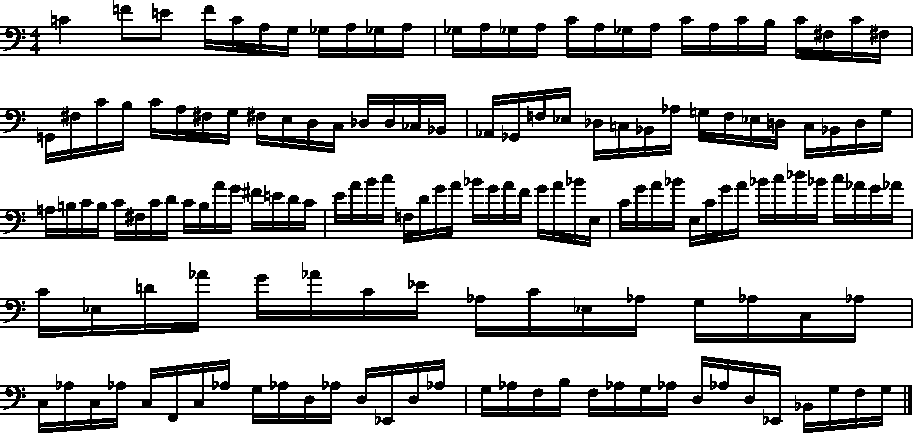
\includegraphics[width=\linewidth]{figures/markov_melody_1.pdf}
	\caption{A melody generated by Markov chains.}
	\label{fig:music:markov1}
\end{figure}

\begin{figure}[h]
	\centering
	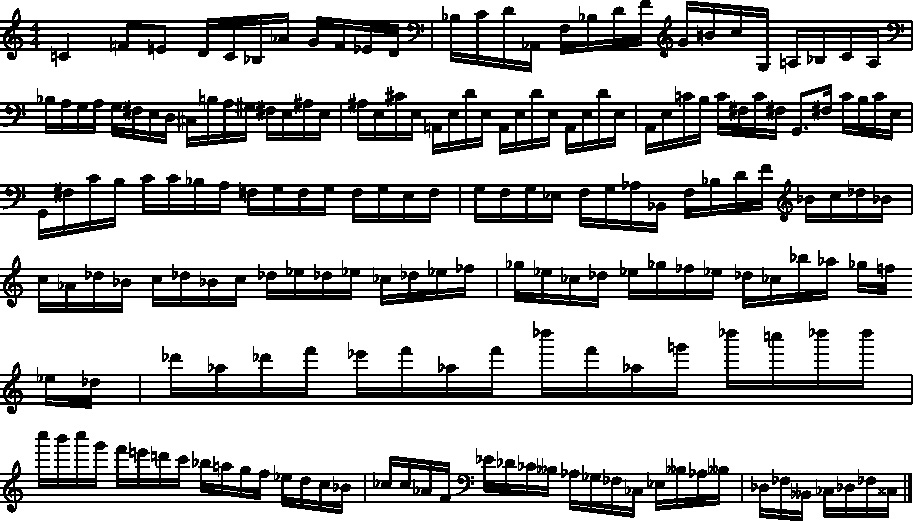
\includegraphics[width=\linewidth]{figures/markov_melody_2.pdf}
	\caption{A melody generated by Markov chains.}
	\label{fig:music:markov2}
\end{figure}

Figures \ref{fig:music:markov1} and \ref{fig:music:markov2} show two melodies generated using Markov chains.
They were generated using a third order Markov chain for the intervals between notes and a second order Markov chain for the rhythms.
Of particular interest, the second measure of the second line of Figure \ref{fig:music:markov2} contains a figure repeated three times.
Additionally, the first measure of the last line of that particular melody contains a perfect run down the B$\flat$ Major scale (from B$\flat$5 to B$\flat$4) in its last two beats.
With the exception of the $E6$ in the second beat of this measure not being an E$\flat$, it is almost a perfect run down the scale starting on G6 and ending on B$\flat$4.

% TODO include figures of randMarkov melodies  (3 & 4 on desktop)

\begin{figure}[h]
	\centering
	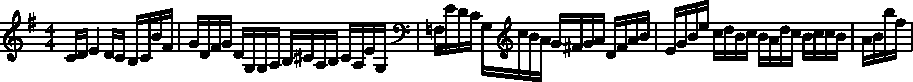
\includegraphics[width=\linewidth]{figures/genetic_melody_1.pdf}
	\caption{A melody generated with the genetic algorithm.}
	\label{fig:music:genetic}
\end{figure}

The melody is Figure \ref{fig:music:genetic} was generated using the genetic algorithm with the surrogate fitness function trained using the chorales from music21's built in corpus of Bach music and an initial population of randomly generated melodies.
Of particular interest in the melody is the set of arpeggiations in the third and fourth measures.
Without explicitly telling the algorithm anything about arpeggiating or repeating ideas in slightly differing ways, it picked up that this makes for good (Bach-like) music.

\begin{figure}[h]
	\centering
	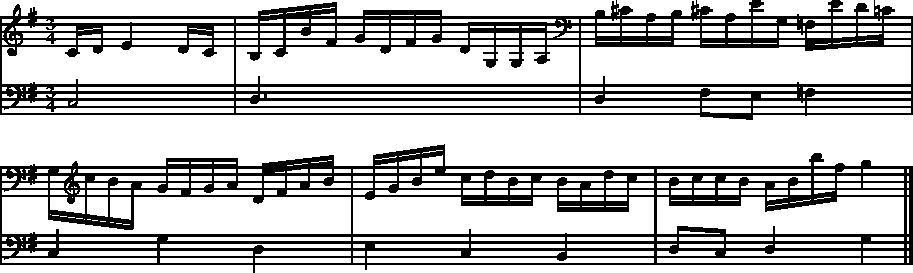
\includegraphics[width=\linewidth]{figures/genetic_melody_1_harmonized.pdf}
	\caption{The melody in Figure \ref{fig:music:genetic} with a bass line written by the author.}
	\label{fig:music:geneticHarmonized}
\end{figure}

Figure \ref{fig:music:geneticHarmonized} showcases one of the potential use cases for the melody generation: compositional inspiration.
The author added a simple bass line to the melody from Figure \ref{fig:music:genetic}, as well as added a more satisfying ending.
% TODO mention work using this melody in Music Tech?

An application of this project is to provide inspiration for the composer.
See Figure \ref{fig:music:geneticHarmonized} for an example where the author used the melody from Figure \ref{fig:music:genetic} and added a bass line.
The generated melodies could also be chained together to create longer compositions, or have their rhythms increased by some multiple to have more than a snippet of music.

The ambitious musician might use these melodies to practice their sight reading; it is extremely unlikely that a melody produced by wither the Markov chains of genetic algorithm has even been written before, let alone seen by a particular musician.
Therefore, these melodies could provide a great opportunity to practice reading music seen for the first time.

\section{Future Work} \label{future}

The work in this project could be expanded by writing code to generate counterpoint or harmonizations of the melodies created using the existing Markov and genetic processes.
One possible method to do this might involve simply using music21's ability to create a \textit{Roman numeral analysis} (RNA) of a piece to determine which chords to use.
Then, the software could fill in the bass, tenor, and alto parts with notes that fit the RNA.
This would likely create very simple, possibly boring, harmonies that may not follow all the voice leading rules of Western music, but it would create \textit{a} complete harmonization.

Many authors have written about the topic of automatic harmonization.
Interestingly, much of the research of this topic focuses on using genetic algorithms to accomplish the task.
William Schottstaedt \cite{schottstdaet_automatic_1989}, defines a genetic algorithm to generate multi-voice music that follows the rules of the Common Practice era.
Somnuk Phon-Amnuaisuk and Geraint A. Wiggins \cite{phon-amnuaisuk_four-part_1999} use genetic algorithms to harmonize preexisting soprano parts.
Andres Acevedo \cite{acevedo_fugue_2004} uses genetic algorithms to write counterpoint in a fugue setting.
A fugue is a music writing technique in which an initial theme is introduced in one part, which is imitated in other parts and repeated throughout the piece.
There are many other examples of using genetic algorithms to solve harmonization and counterpoint; these are just a small sample of the approaches explored.

Other approaches than using genetic algorithms exist for creating pleasing counterpoint.
For example, David Cope discusses a rule based approach to writing counterpoint \cite{cope_computers_1991}.
In this method, a set of rules about how to compose is provided to the program, rather than the program learning from the music on which it is based.
In another approach, Kamil Adiloglu and Ferda Alpaslan \cite{adiloglu_machine_2007} use a feed forward neural network to accept a single voice melody and produce a second voice to complement the first one.

Along with adding counterpoint or harmony generation, other machine learning approaches, one might take different approaches to produce melodies.
For example, Chun-Chi Chen and Risto Miikkulainen \cite{chen_creating_2001} combine neural networks and genetic algorithms by using an evolutionary algorithm to find neural networks that produce good melodies.

% By expanding this project, its use could go beyond merely providing musical inspiration to the composer; it could create entire works, complete with a melody, bass line, and parts in between.
